% Title: gl2ps_renderer figure
% Creator: GL2PS 1.4.0, (C) 1999-2017 C. Geuzaine
% For: Octave
% CreationDate: Thu Apr 29 22:37:34 2021
\setlength{\unitlength}{1pt}
\begin{picture}(0,0)
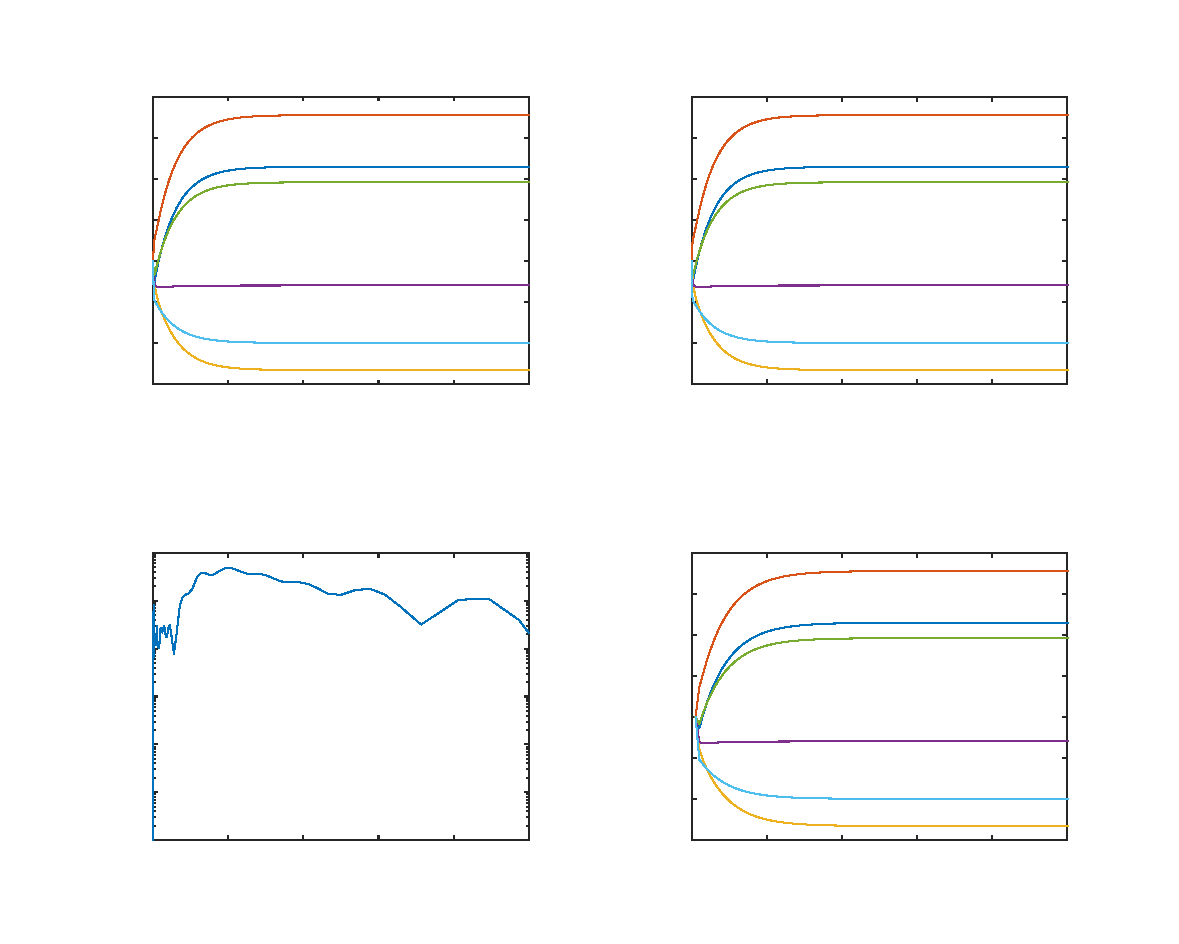
\includegraphics{Trajectory-inc}
\end{picture}%
\begin{picture}(566,453)(0,0)
\fontsize{10}{0}
\selectfont\put(73.5801,261.175){\makebox(0,0)[t]{\textcolor[rgb]{0.15,0.15,0.15}{{0}}}}
\fontsize{10}{0}
\selectfont\put(109.612,261.175){\makebox(0,0)[t]{\textcolor[rgb]{0.15,0.15,0.15}{{20}}}}
\fontsize{10}{0}
\selectfont\put(145.644,261.175){\makebox(0,0)[t]{\textcolor[rgb]{0.15,0.15,0.15}{{40}}}}
\fontsize{10}{0}
\selectfont\put(181.676,261.175){\makebox(0,0)[t]{\textcolor[rgb]{0.15,0.15,0.15}{{60}}}}
\fontsize{10}{0}
\selectfont\put(217.708,261.175){\makebox(0,0)[t]{\textcolor[rgb]{0.15,0.15,0.15}{{80}}}}
\fontsize{10}{0}
\selectfont\put(253.739,261.175){\makebox(0,0)[t]{\textcolor[rgb]{0.15,0.15,0.15}{{100}}}}
\fontsize{10}{0}
\selectfont\put(68.5757,268.672){\makebox(0,0)[r]{\textcolor[rgb]{0.15,0.15,0.15}{{-2}}}}
\fontsize{10}{0}
\selectfont\put(68.5757,288.379){\makebox(0,0)[r]{\textcolor[rgb]{0.15,0.15,0.15}{{-1}}}}
\fontsize{10}{0}
\selectfont\put(68.5757,308.086){\makebox(0,0)[r]{\textcolor[rgb]{0.15,0.15,0.15}{{0}}}}
\fontsize{10}{0}
\selectfont\put(68.5757,327.793){\makebox(0,0)[r]{\textcolor[rgb]{0.15,0.15,0.15}{{1}}}}
\fontsize{10}{0}
\selectfont\put(68.5757,347.5){\makebox(0,0)[r]{\textcolor[rgb]{0.15,0.15,0.15}{{2}}}}
\fontsize{10}{0}
\selectfont\put(68.5757,367.207){\makebox(0,0)[r]{\textcolor[rgb]{0.15,0.15,0.15}{{3}}}}
\fontsize{10}{0}
\selectfont\put(68.5757,386.913){\makebox(0,0)[r]{\textcolor[rgb]{0.15,0.15,0.15}{{4}}}}
\fontsize{10}{0}
\selectfont\put(68.5757,406.62){\makebox(0,0)[r]{\textcolor[rgb]{0.15,0.15,0.15}{{5}}}}
\fontsize{11}{0}
\selectfont\put(163.66,416.62){\makebox(0,0)[b]{\textcolor[rgb]{0,0,0}{{gsl solution in C}}}}
\fontsize{11}{0}
\selectfont\put(54.5757,337.646){\rotatebox{90}{\makebox(0,0)[b]{\textcolor[rgb]{0.15,0.15,0.15}{{x(t)}}}}}
\fontsize{11}{0}
\selectfont\put(163.66,248.175){\makebox(0,0)[t]{\textcolor[rgb]{0.15,0.15,0.15}{{t}}}}
\fontsize{10}{0}
\selectfont\put(332.071,261.175){\makebox(0,0)[t]{\textcolor[rgb]{0.15,0.15,0.15}{{0}}}}
\fontsize{10}{0}
\selectfont\put(368.103,261.175){\makebox(0,0)[t]{\textcolor[rgb]{0.15,0.15,0.15}{{20}}}}
\fontsize{10}{0}
\selectfont\put(404.134,261.175){\makebox(0,0)[t]{\textcolor[rgb]{0.15,0.15,0.15}{{40}}}}
\fontsize{10}{0}
\selectfont\put(440.166,261.175){\makebox(0,0)[t]{\textcolor[rgb]{0.15,0.15,0.15}{{60}}}}
\fontsize{10}{0}
\selectfont\put(476.198,261.175){\makebox(0,0)[t]{\textcolor[rgb]{0.15,0.15,0.15}{{80}}}}
\fontsize{10}{0}
\selectfont\put(512.23,261.175){\makebox(0,0)[t]{\textcolor[rgb]{0.15,0.15,0.15}{{100}}}}
\fontsize{10}{0}
\selectfont\put(327.066,268.672){\makebox(0,0)[r]{\textcolor[rgb]{0.15,0.15,0.15}{{-2}}}}
\fontsize{10}{0}
\selectfont\put(327.066,288.379){\makebox(0,0)[r]{\textcolor[rgb]{0.15,0.15,0.15}{{-1}}}}
\fontsize{10}{0}
\selectfont\put(327.066,308.086){\makebox(0,0)[r]{\textcolor[rgb]{0.15,0.15,0.15}{{0}}}}
\fontsize{10}{0}
\selectfont\put(327.066,327.793){\makebox(0,0)[r]{\textcolor[rgb]{0.15,0.15,0.15}{{1}}}}
\fontsize{10}{0}
\selectfont\put(327.066,347.5){\makebox(0,0)[r]{\textcolor[rgb]{0.15,0.15,0.15}{{2}}}}
\fontsize{10}{0}
\selectfont\put(327.066,367.207){\makebox(0,0)[r]{\textcolor[rgb]{0.15,0.15,0.15}{{3}}}}
\fontsize{10}{0}
\selectfont\put(327.066,386.913){\makebox(0,0)[r]{\textcolor[rgb]{0.15,0.15,0.15}{{4}}}}
\fontsize{10}{0}
\selectfont\put(327.066,406.62){\makebox(0,0)[r]{\textcolor[rgb]{0.15,0.15,0.15}{{5}}}}
\fontsize{11}{0}
\selectfont\put(422.15,416.62){\makebox(0,0)[b]{\textcolor[rgb]{0,0,0}{{analytical solution}}}}
\fontsize{11}{0}
\selectfont\put(313.066,337.646){\rotatebox{90}{\makebox(0,0)[b]{\textcolor[rgb]{0.15,0.15,0.15}{{$x(t)$}}}}}
\fontsize{11}{0}
\selectfont\put(422.15,248.175){\makebox(0,0)[t]{\textcolor[rgb]{0.15,0.15,0.15}{{$t$}}}}
\fontsize{10}{0}
\selectfont\put(73.5801,42.333){\makebox(0,0)[t]{\textcolor[rgb]{0.15,0.15,0.15}{{0}}}}
\fontsize{10}{0}
\selectfont\put(109.612,42.333){\makebox(0,0)[t]{\textcolor[rgb]{0.15,0.15,0.15}{{20}}}}
\fontsize{10}{0}
\selectfont\put(145.644,42.333){\makebox(0,0)[t]{\textcolor[rgb]{0.15,0.15,0.15}{{40}}}}
\fontsize{10}{0}
\selectfont\put(181.676,42.333){\makebox(0,0)[t]{\textcolor[rgb]{0.15,0.15,0.15}{{60}}}}
\fontsize{10}{0}
\selectfont\put(217.708,42.333){\makebox(0,0)[t]{\textcolor[rgb]{0.15,0.15,0.15}{{80}}}}
\fontsize{10}{0}
\selectfont\put(253.739,42.333){\makebox(0,0)[t]{\textcolor[rgb]{0.15,0.15,0.15}{{100}}}}
\fontsize{10}{0}
\selectfont\put(68.5757,49.8301){\makebox(0,0)[r]{\textcolor[rgb]{0.15,0.15,0.15}{{$10^{-9}$}}}}
\fontsize{10}{0}
\selectfont\put(68.5757,72.8213){\makebox(0,0)[r]{\textcolor[rgb]{0.15,0.15,0.15}{{$10^{-8}$}}}}
\fontsize{10}{0}
\selectfont\put(68.5757,95.8125){\makebox(0,0)[r]{\textcolor[rgb]{0.15,0.15,0.15}{{$10^{-7}$}}}}
\fontsize{10}{0}
\selectfont\put(68.5757,118.804){\makebox(0,0)[r]{\textcolor[rgb]{0.15,0.15,0.15}{{$10^{-6}$}}}}
\fontsize{10}{0}
\selectfont\put(68.5757,141.795){\makebox(0,0)[r]{\textcolor[rgb]{0.15,0.15,0.15}{{$10^{-5}$}}}}
\fontsize{10}{0}
\selectfont\put(68.5757,164.786){\makebox(0,0)[r]{\textcolor[rgb]{0.15,0.15,0.15}{{$10^{-4}$}}}}
\fontsize{10}{0}
\selectfont\put(68.5757,187.777){\makebox(0,0)[r]{\textcolor[rgb]{0.15,0.15,0.15}{{$10^{-3}$}}}}
\fontsize{11}{0}
\selectfont\put(163.66,197.777){\makebox(0,0)[b]{\textcolor[rgb]{0,0,0}{{Difference between gsl and analytical solution}}}}
\fontsize{11}{0}
\selectfont\put(22.5757,118.804){\rotatebox{90}{\makebox(0,0)[b]{\textcolor[rgb]{0.15,0.15,0.15}{{$\sum_i |x_i(t) - x_i(t;\texttt{gsl})|$}}}}}
\fontsize{11}{0}
\selectfont\put(163.66,29.333){\makebox(0,0)[t]{\textcolor[rgb]{0.15,0.15,0.15}{{$t$}}}}
\fontsize{10}{0}
\selectfont\put(332.071,42.333){\makebox(0,0)[t]{\textcolor[rgb]{0.15,0.15,0.15}{{0}}}}
\fontsize{10}{0}
\selectfont\put(368.103,42.333){\makebox(0,0)[t]{\textcolor[rgb]{0.15,0.15,0.15}{{20}}}}
\fontsize{10}{0}
\selectfont\put(404.134,42.333){\makebox(0,0)[t]{\textcolor[rgb]{0.15,0.15,0.15}{{40}}}}
\fontsize{10}{0}
\selectfont\put(440.166,42.333){\makebox(0,0)[t]{\textcolor[rgb]{0.15,0.15,0.15}{{60}}}}
\fontsize{10}{0}
\selectfont\put(476.198,42.333){\makebox(0,0)[t]{\textcolor[rgb]{0.15,0.15,0.15}{{80}}}}
\fontsize{10}{0}
\selectfont\put(512.23,42.333){\makebox(0,0)[t]{\textcolor[rgb]{0.15,0.15,0.15}{{100}}}}
\fontsize{10}{0}
\selectfont\put(327.066,49.8301){\makebox(0,0)[r]{\textcolor[rgb]{0.15,0.15,0.15}{{-2}}}}
\fontsize{10}{0}
\selectfont\put(327.066,69.5366){\makebox(0,0)[r]{\textcolor[rgb]{0.15,0.15,0.15}{{-1}}}}
\fontsize{10}{0}
\selectfont\put(327.066,89.2437){\makebox(0,0)[r]{\textcolor[rgb]{0.15,0.15,0.15}{{0}}}}
\fontsize{10}{0}
\selectfont\put(327.066,108.95){\makebox(0,0)[r]{\textcolor[rgb]{0.15,0.15,0.15}{{1}}}}
\fontsize{10}{0}
\selectfont\put(327.066,128.657){\makebox(0,0)[r]{\textcolor[rgb]{0.15,0.15,0.15}{{2}}}}
\fontsize{10}{0}
\selectfont\put(327.066,148.364){\makebox(0,0)[r]{\textcolor[rgb]{0.15,0.15,0.15}{{3}}}}
\fontsize{10}{0}
\selectfont\put(327.066,168.071){\makebox(0,0)[r]{\textcolor[rgb]{0.15,0.15,0.15}{{4}}}}
\fontsize{10}{0}
\selectfont\put(327.066,187.777){\makebox(0,0)[r]{\textcolor[rgb]{0.15,0.15,0.15}{{5}}}}
\fontsize{11}{0}
\selectfont\put(422.15,197.777){\makebox(0,0)[b]{\textcolor[rgb]{0,0,0}{{lsode solution in \emph{GNU Octave}}}}}
\fontsize{11}{0}
\selectfont\put(313.066,118.804){\rotatebox{90}{\makebox(0,0)[b]{\textcolor[rgb]{0.15,0.15,0.15}{{$x(t)$}}}}}
\fontsize{11}{0}
\selectfont\put(422.15,29.333){\makebox(0,0)[t]{\textcolor[rgb]{0.15,0.15,0.15}{{$t$}}}}
\end{picture}
